%
% The first command in your LaTeX source must be the \documentclass command.
\documentclass[sigconf,review=true,anonymous=true,screen]{acmart}

\usepackage{algorithmic}
\usepackage[ruled]{algorithm2e}
\usepackage{subcaption}

%
% defining the \BibTeX command - from Oren Patashnik's original BibTeX documentation.
\def\BibTeX{{\rm B\kern-.05em{\sc i\kern-.025em b}\kern-.08emT\kern-.1667em\lower.7ex\hbox{E}\kern-.125emX}}
   
\newcommand{\ignore}[1]{}
\newcommand\norm[1]{\left\lVert#1\right\rVert}
\newcommand{\eps}{\varepsilon}
\renewcommand{\phi}{\varphi}

   
    
% Rights management information. 
% This information is sent to you when you complete the rights form.
% These commands have SAMPLE values in them; it is your responsibility as an author to replace
% the commands and values with those provided to you when you complete the rights form.
%
% These commands are for a PROCEEDINGS abstract or paper.
\copyrightyear{2019}
\acmYear{2019}
\setcopyright{acmlicensed}
\acmConference[KDD '19]{KDD '19: SIGKDD Conference on Knowledge Discovery and Data Mining}{August 04--06, 2019}{Anchorage, AL}
\acmBooktitle{KDD '19: SIGKDD Conference on Knowledge Discovery and Data Mining, Aug 04--06, 2019, Anchorage, AL}
%\acmPrice{15.00}
%\acmDOI{10.1145/1122445.1122456}
%\acmISBN{978-1-4503-9999-9/18/06}

%
% These commands are for a JOURNAL article.
%\setcopyright{acmcopyright}
%\acmJournal{TOG}
%\acmYear{2018}\acmVolume{37}\acmNumber{4}\acmArticle{111}\acmMonth{8}
%\acmDOI{10.1145/1122445.1122456}

%
% Submission ID. 
% Use this when submitting an article to a sponsored event. You'll receive a unique submission ID from the organizers
% of the event, and this ID should be used as the parameter to this command.
%\acmSubmissionID{123-A56-BU3}

%
% The majority of ACM publications use numbered citations and references. If you are preparing content for an event
% sponsored by ACM SIGGRAPH, you must use the "author year" style of citations and references. Uncommenting
% the next command will enable that style.
%\citestyle{acmauthoryear}

%
% end of the preamble, start of the body of the document source.
\begin{document}

%
% The "title" command has an optional parameter, allowing the author to define a "short title" to be used in page headers.
\title{New Heavy Hitters Algorithms with Tail Bounds}

%
% The "author" command and its associated commands are used to define the authors and their affiliations.
% Of note is the shared affiliation of the first two authors, and the "authornote" and "authornotemark" commands
% used to denote shared contribution to the research.
\author{Arnab Bhattacharyya}
\author{Sharanya Chakravarthi}
\author{Tejas Kaushik}
\author{Ashish Kumar Sen}
%
% By default, the full list of authors will be used in the page headers. Often, this list is too long, and will overlap
% other information printed in the page headers. This command allows the author to define a more concise list
% of authors' names for this purpose.
\renewcommand{\shortauthors}{Bhattacharyya et al.}

%
% The abstract is a short summary of the work to be presented in the article.
\begin{abstract}
In a stream of $m$ items belonging to $\{1, \dots, n\}$, the {\em $(\eps, \phi)$-Heavy Hitters} problem is to output a set $S$ of items containing all items of frequency $\geq \phi m$ and no item of frequency $< (\phi-\eps)m$. It is one of the most heavily-studied problems in data streams, with a wide variety of applications. 

In this work, we propose new randomized counter-based algorithms for the heavy-hitters problem. We show that not only do they have nearly optimal space complexity with respect to $\eps, \phi,$ and $n$, they also exhibit strong error bounds in terms of the frequency tail of the input and perform favorably on realistic data sets.
\end{abstract}

%
% The code below is generated by the tool at http://dl.acm.org/ccs.cfm.
% Please copy and paste the code instead of the example below.
%
\begin{CCSXML}
<ccs2012>
<concept>
<concept_id>10002951.10003227.10003351</concept_id>
<concept_desc>Information systems~Data mining</concept_desc>
<concept_significance>500</concept_significance>
</concept>
<concept>
<concept_id>10003752.10003809</concept_id>
<concept_desc>Theory of computation~Design and analysis of algorithms</concept_desc>
<concept_significance>300</concept_significance>
</concept>
<concept>
<concept_id>10003033.10003099.10003105</concept_id>
<concept_desc>Networks~Network monitoring</concept_desc>
<concept_significance>100</concept_significance>
</concept>
</ccs2012>
\end{CCSXML}

\ccsdesc[500]{Information systems~Data mining}
\ccsdesc[300]{Theory of computation~Design and analysis of algorithms}
\ccsdesc[100]{Networks~Network monitoring}
%
% Keywords. The author(s) should pick words that accurately describe the work being
% presented. Separate the keywords with commas.
\keywords{data streaming, frequent items, randomized algorithms}

%
% A "teaser" image appears between the author and affiliation information and the body 
% of the document, and typically spans the page. 

%
% This command processes the author and affiliation and title information and builds
% the first part of the formatted document.
\maketitle

\section{Introduction}
\subsection{Background}
The {\em data streaming} model is an important tool for analyzing algorithms on massive data sets \cite{Muthu05}. Streaming algorithms
take a long stream of items as input and produce a compact summary of the data as output. This summary can be used to answer queries about the properties of the input data stream. The algorithms are often constrained to take a single pass over the data.

A concrete application is the problem of monitoring IP network traffic. Here, data stream management systems monitor IP packets sent on communication links and perform detailed statistical analyses. These analyses are crucial for fault diagnoses and for verifying network performance and security. Examples of such systems are Gigascope at AT\&T \cite{Giga} and CMON at Sprint \cite{CMON}. The main challenge in these systems is to quickly and accurately perform the needed analyses in the face of a very high rate of updates.


In this work, we consider the {\em heavy-hitters} problem. Informally, the goal is to find the frequent elements in the stream; the same problem is also studied under the names of top-k, popular items, frequent items, elephants, or iceberg queries. It is very heavily studied and commonly used, e.g. in network analyses to find addresses that account for a large fraction of a network link utilization in a given time window. It is also often solved as a subroutine within more advanced data stream computations, e.g. approximating the entropy of a stream. Cormode and Hadjieleftheriou in \cite{FrequentSurvey} give an excellent survey of the work on this problem in a unified framework. 

We formulate the heavy-hitters problem rigorously as follows:
\begin{definition}\label{def:hh}
    In the {\em $(\varepsilon, \varphi)$-Heavy Hitters Problem}, we are given
    parameters $0< \varepsilon <\varphi$ $\leqslant$ 1 and a stream $a_{1},....,a_{m}$
    of items $a_{j}$ in $\left\{1,2,.....n\right\}$. Let $f_{i}$ denote the number of
    occurrences of item $i$, i.e., its frequency\footnote{We assume throughout this paper that there are only insertions (no deletion) in the stream and that each insertion of an item increases its frequency by $1$. }. An algorithm for the problem should make one pass over the stream and at the end
    of the stream output a set $S \subseteq \left\{1,2,.....n\right\}$ which contains any $i$ such that $f_i \geq \phi m$ and does not contain any $i$ such that $f_i < (\phi - \eps)m$.
 
 Furthermore, for each item $i\in S$, the algorithm should output an estimate $\tilde{f_{i}}$ of the frequency $f_{i}$ which satisfies $|f_{i} -\tilde{f_{i}}|$ $ \leqslant \varepsilon m$. 
\end{definition}
    A large number of algorithms have been proposed for finding the heavy hitters and their variants. Following \cite{FrequentSurvey}, they can be broadly classified into {\em Counter-based} algorithms, {\em Quantile} Algorithms,  and {\em Sketch} algorithms. 

    One of the first algorithms for the problem, as well as perhaps the most widely used, is the deterministic counter-based \textsc{Frequent} algorithm  due to Misra and Gries \cite{MG82} (independently re-discovered 20 years later with some refinements to the implementation by Karp et al. \cite{KSP03} and Demaine et al. \cite{DLM02}). There are several variants of the algorithm, notably \textsc{LossyCounting} \cite{MM02} and \textsc{SpaceSaving} \cite{MAA05}, that sometimes perform better in terms of space usage or update time than the original version. All these algorithms use $O(\eps^{-1}(\log n + \log m))$ bits of space; note the bound does {\em not} depend on $\varphi$. Sketching algorithms, such as the CountSketch \cite{CCF02} or the Count-Min Sketch \cite{CM05}, require more storage (but they can handle more general streams with both insertions and deletions that we do not study here).
    
Recently, in \cite{BDW16}, Bhattacharyya et al.~introduced two new algorithms for the $(\eps, \phi)$-heavy hitters problem that improve on the space usage of \textsc{Frequent}, particularly when $\varphi \gg \eps$. One of their algorithms uses $O(\eps^{-1}\log\varphi^{-1}+\varphi^{-1} \log n + \log \log m)$ bits of storage, which is optimal upto constant factors. Moreover, the algorithms take a constant amount of time per update. These algorithms are fundamentally counter-based and use the Misra-Gries algorithm as a subroutine, but they also use random sampling and hashing in crucial ways.

\subsection{Our Work}
Given the strong theoretical guarantees of the algorithms proposed in \cite{BDW16}, it is natural to wonder how well they fare in practice. 

Berinde et al.~\cite{BCIS} observe that one of the main reasons for the real-world success of \textsc{Frequent} is that it displays ``better-than-advertised'' performance on streams which have a {\em skewed} frequency distribution. In particular, they showed that the error made by \textsc{Frequent} in frequency estimation satisfies a ``tail bound'', so that it is very small when heavy hitters constitute most of the stream.

The starting point of this work is the observation that the algorithms proposed in \cite{BDW16} do {\em not} exhibit a tail bound, so that the estimation error can be large even when the frequency distribution is very skewed. We design new randomized algorithms inspired by \cite{BDW16} that improve \textsc{Frequent} in terms of bits of storage while still achieving a tail bound. We show two different algorithms with this feature. Although they are novel to the best of our knowledge, they are both quite simple to implement and analyze. The first algorithm combines a \textsc{Frequent} data structure with a Count-Min sketch \cite{CM05}. The second algorithm maintains two \textsc{Frequent} data structures, one with a smaller number of counters containing items from the original universe and another with a larger number of counters recording hashes of the original item id's.
Armed with the tail guarantee and following the analysis of Berinde et al.~\cite{BCIS}, we then show that our proposed algorithms enjoy several other appealing properties, such as guarantees for skewed Zipfian streams, for the sparse recovery problem and for merging multiple streams.

We experimentally evaluate $\dots$.




    \section{Preliminaries}
    \subsection{General}
For a stream consisting of $m$ insertions from the universe $[n] \coloneqq \{1,\dots, n\}$, we let the $n$-dimensional vector $f = (f_1, \dots, f_n)$
denote the frequencies of the $n$ items. So, $\sum_{i=1}^n f_i = m$. Without loss of generality, we will assume that $f_1 \geq f_2 \geq \cdots \geq f_n$. 

For any integer $k \geq 0$, the {\em residual $k$-tail} of the stream is defined as\footnote{The 1 in the subscript refers to the fact that this is the 1st moment of the residual stream.}:
$$F_1^{\text{res}(k)} = \sum_{i=k+1}^n f_i.$$
That is, the residual $k$-tail is the sum of the frequencies except the $k$ largest ones. 

Recall from Definition \ref{def:hh} that an algorithm for the $(\eps, \varphi)$-heavy hitters problem is supposed to output estimates $\tilde{f}_i$ for each $i$ in the output set such that:
$$|\tilde{f}_i - f_i| \leq \eps \cdot m = \eps\cdot F_1^{\text{res}(0)}.$$
\begin{definition}[Tail Bound]\label{def:tailbd}
An algorithm for the $(\eps,\varphi)$-heavy hitters problem is said to satisfy the {\em $K$-tail bound} if for every $0\leq k\leq K$:
$$|\tilde{f}_i - f_i| \leq \eps \cdot F_1^{\text{res}(k)}$$
for all $i$ in the output set of the algorithm.
\end{definition}
The larger the $K$ we can get for the tail bound, the stronger is the obtained guarantee. 


Our proposed algorithms use the notion of a {\em universal hash family}, which we define next.
\begin{definition}
A family $\mathcal{H}$ consisting of functions $h: U \to [m]$ is said to be a {\em universal hash family} if 
for all distinct $x, y \in U$:
$$\Pr_{h \leftarrow \mathcal{H}}[h(x)=h(y)] \leq \frac1m$$
where the probability is over $h$ drawn uniformly at random from $\mathcal{H}$. 
\end{definition}
It is folklore that if $m \leq |U|$, there exists a universal hash family whose members can be represented uniquely using $O(\log |U|)$ bits.

\subsection{The \textsc{Frequent} algorithm}   
    \begin{algorithm}
    	\caption{\textsc{Frequent}, \cite{MG82}}
	\label{fig:freq}
    	\SetAlgoLined
	\SetKwProg{Fn}{Function}{}{}
	
	\KwData{Number of counters $t$}

	\textbf{Initialization:}
\Begin{
	Empty set $T $\\
Empty array $c$ of length $n$\\
 }   	
	\Fn{Insert(i)}{
    	\If{$i \in T$}{
    	$c_i \leftarrow c_i + 1$;\\
	}
    	\ElseIf{$|T| < t$} {
    	 $T \leftarrow T \cup \{i\}$;\\
    	$c_i \leftarrow 1$;\\
}
	\Else{
    	 \ForEach{$j \in T$}{
    	$c_j \leftarrow c_j - 1$;\\
    	\lIf{$c_j = 0$}{$T \leftarrow T\setminus \{j\}$}
}
}
}

	\Fn{Report()}{
	\lForEach{$i \in T$}{Output $(i, c_i)$}
}
    \end{algorithm}

    \vspace*{.5cm}
\textsc{Frequent}, shown in Algorithm \ref{fig:freq}, maintains $t$ (item, counter) pairs. Its reported frequencies are accurate to within $m/(t+1)$ where $m$ is the length of the stream. In particular, it reports all items with frequency at least $m/(t+1)$. 

\ignore{In the algorithm, each new item is compared with stored items and if the new item is among the stored items, then the count value of stored items is incremented. Else, if it is not the one already present and there is some counter whose value is zero, then this item in the table is stored and the counter value is set to one. Else if all counter value is non-zero, then the counter value is decremented by 1 for each item. }
A simple grouping argument can be used to verify the correctness of the algorithm. With $t = \lceil 1/\eps \rceil$ counters, \textsc{Frequent} solves the $(\eps,\phi)$-Heavy hitters problem using $O(\varepsilon^{-1} (\log n + \log m))$ bits of space. Berinde et al.~\cite{BCIS} showed a stronger tail bound:
\begin{theorem}(\cite{BCIS})\label{thm:tailfreq}
For any $t \geq \frac1\eps$, the \textsc{Frequent} algorithm with $t$ counters satisfies the $\left(t-\frac1\eps\right)$-tail bound and uses $O(t(\log n + \log m))$ bits of storage.
\end{theorem}
\ignore{
We sketch an analysis of the error bound present in Berinde et al. \cite{BCIS}. 
The \textsc{Frequent} algorithm can be interpreted in the following way:
    each element in the stream results in incrementing one counter, and the insertion of some $d$ elements cause $t+1$ counters to be decremented (including the implicit decrement of the item being inserted). The sum
    of the counters at the end of the algorithm is $\norm{c}_1$. We have
   		 $\norm{c}_1 = \norm{f}_1 - d(t+1)$.
  Note that the final counter value for any element is at least  $f_i - d$. Restricting our attention to the $k$ most frequent elements\footnote{In fact, the inequality holds for {\em any} set of $k$ elements.} (which are without loss of generality, $\{1, \dots, k\}$): 
    $$\norm{c}_1 = \norm{f}_1 - d(t+1) \geq \sum_{i=1}^k(f_i-d).$$
 Therefore:
\begin{equation}
d \leq \sum_{i=k+1}^n f_i/(t-k+1)
\end{equation}
Since the error $\delta_i := f_i - c_i$ is at most $d$, by setting $k = 0$ in the above, for any $i \in [n]$:
\begin{equation}\label{eqn:std_freq}
\delta_i \leq m/(t+1)
\end{equation}
More strongly, if $F_1^{\text{res}(k)}$ is the top-$k$ residual $\sum_{i=k+1}^n f_i$, we get for any $i \in [n]$:
\begin{equation}\label{eqn:freq_tail}
\delta_i \leq F_1^{\text{res}(k)}/(t - k+1)
\end{equation}
Berinde et al.~\cite{BCIS} call a bound of the form (\ref{eqn:freq_tail}) a {\em $k$-tail guarantee}. 
Streams in real-life often display a characteristically skewed frequency distribution, with the heavy hitters
constituting a large fraction of the stream. A residual tail guarantee is in this case asymptotically better than a uniform guarantee.
As we describe later, Berinde et al.~also show that a $k$-tail guarantee implies bounds for {sparse recovery}, stronger error bounds for streams with Zipfian frequency distribution and for mergeability of multiple summaries. These properties make the \textsc{Frequent} algorithm even more useful in practice than what would be suggested just by the bound (\ref{eqn:std_freq}).
}
\subsection{The work of \cite{BDW16}}\label{sec:bdw}
In the recent work \cite{BDW16}, Bhattacharyya, Dey and Woodruff introduce a couple of randomized counter-based algorithms that improve upon \textsc{Frequent} in terms of the number of bits needed for storage. Their first algorithm solves the $(\eps,\phi)$-Heavy hitters problem with space $O(1/\eps \log 1/\eps + 1/\phi \log n + \log \log m)$ bits, while their second algorithm uses $O(1/\eps \log 1/\phi + 1/\phi \log n + \log \log m)$ bits. When $\eps \ll \phi$, the space requirement for these algorithms is asymptotically smaller than the worst-case space requirement for \textsc{Frequent}. In fact, \cite{BDW16} show that the second algorithm achieves the optimal (up to constant factors) number of bits for solving the $(\eps, \phi)$-Heavy hitters problem.

The first algorithm of \cite{BDW16}, which we dub \textsc{CompressedFrequent}, is shown below as Algorithm \ref{fig:alg1}. \textsc{CompressedFrequent} runs Misra and Gries' \textsc{Frequent} algorithm on a sampled stream of length $O(1/\eps^2)$ on a hashed universe of size $O(1/\eps^4)$. By the choice of parameters, there are no hash collisions among the elements sampled from the stream with high probability. Also, by standard concentration results, the relative frequency of any element in the original stream and the sampled stream differ by at most $\eps/2$. Some additional bookkeeping needs to be done to ensure that we have the original (unhashed) id's of the heavy hitters, but otherwise, the analysis is complete.


    \begin{algorithm}
    	\caption{\textsc{CompressedFrequent}, \cite{BDW16}}
	\label{fig:alg1}
    	\SetAlgoLined
	\SetKwProg{Fn}{Function}{}{}
	
	\KwData{Parameters $\eps$ and $\phi$ with $0<\eps\leq\phi<1$.}


\ignore{
    	\textbf{Input:} A stream S of length m over universe $\mathcal{U}=[n]$; let f(x) be the frequency of $x\in \mathcal{U}$ in S\\
    	\textbf{Output:} A set $X \subseteq U$ and a function $\tilde{f} : X \rightarrow N$ such that if $f(x)\geqslant \varphi m$, then $x \in X$ and 
    	$f(x)- \varepsilon m \leqslant \tilde{f(x)} \leqslant f(x) + \varepsilon m$ and if $f(y) \leqslant \varphi m$, then y  $\notin X $  for every x, y $\in \mathcal{U}$\\
}    	
 \textbf{Initialization:}
\Begin{
$\ell \leftarrow 6\log(6/\delta)/\varepsilon^{2}$.\\ 
Hash function $h$ drawn uniformly from a universal family $H \subseteq \left\{[n] \rightarrow 
    	[4\ell^{2}/\delta ] \right\}.$ \\
An empty \textsc{Frequent} data structure $\mathcal{T}_{1}$ with $\varepsilon^{-1}$ counters. \\
\ignore{Each key entry of $\mathcal{T}_{1}$ can store \hspace*{.5cm} an integer of $[0,\lceil{400l^2/\delta}\rceil]$ and each value \hspace*{.6cm}entry can store an integer in $[0,11\ell]$. The \hspace*{.6cm}Table $\mathcal{T}_{1}$ will be in sorted order by value \hspace*{.6cm}throughout}
An empty set $\mathcal{T}_{2}$. \\
\ignore{Each \hspace*{.5cm}entry of $\mathcal{T}_{2}$ can store an integer in $[0,n]$. \hspace*{.5cm}The entries of $\mathcal{T}_{2}$ will correspond to ids of \hspace*{.5cm}the keys in $\mathcal{T}_{1}$ of the highest $1/\varphi$ values}
}
    
\Fn{Insert($x$)}{
 With probability $6\ell/m $, \textbf{continue}. Else, \KwRet\;
Call Insert($h(x)$) on $\mathcal{T}_1$\;
%,m     	9: Perform Misra-Gries update using $h(x)$ \hspace*{.4cm} maintaining $\mathcal{T}_{1}$ sorted by values.\\
  \If{$h(x)$ is among the  top $1/\varphi$ valued items in $\mathcal{T}_{1}$}{
\If{$x \not \in \mathcal{T}_{2}$}{
 \eIf{$|\mathcal{T}_{2}| = 1/\phi$}{
For some $y$ in $\mathcal{T}_{2}$ such that $h(y)$ is not among the top $1/\varphi$ valued items in $\mathcal{T}_{1}$, replace $y$ with $x$}
{
Insert $x$ in $\mathcal{T}_{2}$\;  
}
}
}
}
 \Fn{Report()}{
\ForEach{$x$ in $\mathcal{T}_2$}{\lIf{$\mathcal{T}_1[h(x)] \geq (\phi - \eps/2)\ell$}{Output $(x, \mathcal{T}_1[h(x)])$}}
}
    \end{algorithm}
    

The second algorithm of \cite{BDW16} is more intricate. It also operates on $O(1/\eps^2)$ samples from the original stream and then maintains a compressed histogram for hashes of the original items. It is somewhat reminiscent of the Count-Min sketch algorithm of Cormode and Muthukrishnan \cite{CM05}, but it also subsamples items from the sample with subsampling rate tuned to a mutliplicative approximation of the frequency. We omit a more detailed description of this algorithm because we do not study it in this work.

\ignore{
	\section{Our Contribution: Tail guarantees for randomized counter-based solutions}

We begin by observing that the randomized counter-based algorithms from \cite{BDW16}, described above in Section \ref{sec:bdw}, cannot admit a tail guarantee, like the bound in (\ref{eqn:freq_tail}) shown for \textsc{Frequent}. This is because even if the stream only has two types of elements, so that $F_1^{\text{res}(2)} = 0$, there will still be some error in the frequency approximation from the sampling step. So, random sampling cannot be used as a technique if we want to retain the tail guarantee of \textsc{Frequent}. 

In this work, we show that we can improve \textsc{Frequent} in terms of bits of storage while still achieving the $k$-tail guarantee. We show two different algorithms with this feature. Although they are novel to the best of our knowledge, they are both quite simple to implement and analyze. The first algorithm combines a \textsc{Frequent} data structure with a Count-Min sketch \cite{CM05}. The second algorithm maintains two \textsc{Frequent} data structures, one with a smaller number of counters containing items from the original universe and another with a larger number of counters recording hashes of the original item id's.

Armed with the tail guarantee and following the analysis of Berinde et al.~\cite{BCIS}, we can then show that our proposed algorithms enjoy several other appealing properties, such as guarantees for skewed Zipfian streams, for the sparse recovery problem and for merging multiple streams.
}
\section{New Algorithms}
We start with the observation that the algorithms proposed in \cite{BDW16} cannot satisfy a non-trivial tail guarantee. Consider the \textsc{CompressedFrequent} algorithm shown in Figure \ref{fig:alg1}, and suppose the input stream only consists of two items with each inserted $\Omega(m)$ times. Although $F_1^{\text{res}(2)}=0$, the frequency estimates output by the algorithm will still have nonzero error because due to random sampling, the relative frequency of the two items in the sampled stream will (with high probability) differ from that in the original stream. The same argument holds for the second algorithm of \cite{BDW16}.

\subsection{\textsc{SketchFrequent}}
 	\begin{algorithm}
		\caption{\textsc{SketchFrequent}}
    	\SetAlgoLined
	\SetKwProg{Fn}{Function}{}{}

	\KwData{Width $w$, Input parameters $\phi, \delta \in (0,1)$.}


\textbf{Initialization}:
\Begin{
$\ell \leftarrow \log(4/\delta\phi)$\\
Hash functions $h_1, \dots, h_\ell$ drawn uniformly from a universal family $H \subseteq \left\{[n] \to [w] \right\}.$ \\
Empty \textsc{Frequent} data structure $\mathcal{T}$ with $2/\phi$ counters.\\
Empty matrix $\mathcal{C}$ with $\ell$ rows and $w$ columns.
}
\Fn{Insert($x$)}{
Insert $x$ into $\mathcal{T}$\;
\For{$i = 1$ to $\ell$}
{Increment $\mathcal{C}[i][h_i(x)]$\;}
}
\Fn{Report()}{
\ForEach{$x \in \mathcal{T}$}{
$\hat{f}_x \leftarrow \min_{i \in [\ell]} \mathcal{C}[i][h_i(x)]$\;
\If{$\hat{f}_x \geq \phi m$}{
Output $(x,\hat{f}_x)$\;
}}}
	\end{algorithm}
Our first algorithm, shown above, runs the Count-Min sketch on the output of a \textsc{Frequent} counter solving the $(\phi,\phi/2)$-Heavy hitters problem.

\begin{theorem}
Let $\ell = \log(4/\delta \varphi)$ as in the algorithm above.  Suppose that $\eps < \frac{\varphi^2 \delta}{2\ell}$. 

For any $w \geq \frac2\eps$ and $\delta \in [0,1]$,  \textsc{SketchFrequent} satisfies the $\sqrt{\frac{\delta w}{\ell}}$-tail bound with probability $1-\delta$ 
and uses 
$O(\varphi^{-1} \log n + w \log (\delta\phi)^{-1} \log m)$ bits of storage.

In particular, for $w = \frac2\eps$ and $\delta=\frac15$, \textsc{SketchFrequent} solves the $(\eps,\phi)$-heavy hitters problem with probability at least $\frac45$ using $O(\varphi^{-1}\log n + \eps^{-1} \log \phi^{-1} \log m)$ bits\footnote{The assumption that $\eps <\varphi^2\delta/2\ell$ is not needed for the last part of the theorem.}.
\ignore{
solves the $(\phi, \eps)$-Heavy hitters problem. In particular, for any $0 \leq k \leq \sqrt{\delta w/\ell}$, with probability at least $1-\delta$, for any $(x, \hat{f}_x)$ reported by the algorithm,
$$0 \leq \hat{f}_x - f_x \leq \eps F_1^{\text{res}(k)}.$$
The algorithm uses $O(\phi^{-1} \log  n + \eps^{-1} \log \phi^{-1} \log m)$ bits of storage.}
\end{theorem}
\begin{proof}The space complexity is immediate. We will focus on the tail bound.
We argue first that on the top $k=\sqrt{\delta w/\ell}$ elements of the stream, $h_1, \dots, h_\ell$ do not collide with probability at least $1-\delta/2$.
\begin{lemma}
Let $k = \sqrt{\delta w/\ell}$. For any fixed $T \subseteq [n]$ of size $k$,
$$\Pr[\exists i \in [\ell], \exists x \neq y \in T, h_j(x)=h_j(y)] < \delta/2.$$
\end{lemma}
\begin{proof}
By definition of a universal hash family, for any fixed $i \in [\ell]$ and $x \neq y \in T$, $\Pr[h_i(x)=h_i(y)]<1/w$. Using the union bound:
$$\Pr[\exists i \in [\ell], \exists x \neq y \in T, h_i(x)=h_i(y)] \leq \ell \cdot {t \choose 2} \cdot \frac1w < \frac{\delta}{2}$$
\end{proof}
Condition on the above event. Note that by our assumption, $k>2/\varphi$. We can now run the usual analysis of the count-min sketch, which we reproduce here for completeness. 

Consider an $x \in [n]$ that is stored in one of $\mathcal{T}$'s counters. Because of the above, and using again universality of the hash family, for any $i \in [\ell]$:
$$\mathbb{E}[C[i][h_i(x)]] = f_x + \frac1w\sum_{y>k} f_y = f_x + \frac{F_1^{\text{res}(k)}}{w} \leq f_x + \frac{\eps}{2} F_1^{\text{res}(k)}.$$
Then, by Markov's inequality:
$\Pr[C[i][h_i(x)]-f_x > \eps F_1^{\text{res}(k)}] \leq \frac12$. Therefore:
$$\Pr[\hat{f}_x - f_x > \eps F_1^{\text{res}(k)}] \leq \frac{1}{2^\ell} = \frac{\phi\delta}{4}.$$
Doing a union bound over $\frac2\varphi$ elements shows that with probability at least $1-\delta/2$, for each $x \in \mathcal{T}$,
$\hat{f}_x - f_x \leq \eps F_1^{\text{res}(k)}$. Moreover, observe that every $x$ with $f_x \geq \varphi m$ is output by the algorithm.
\end{proof}

\subsection{\textsc{DoubleFrequent}}

 	\begin{algorithm}
		\caption{\textsc{DoubleFrequent}}
    	\SetAlgoLined
	\SetKwProg{Fn}{Function}{}{}

	\KwData{Number of counters $t$, Input parameters $\eps,\phi, \delta \in (0,1)$ with $\eps\leq\phi/2$.}


\ignore{		\textbf{Input:} A stream S of length m over universe $\mathcal{U}=[n]$; let f(x) be the frequency of $x\in \mathcal{U}$ in S\\
		\textbf{Output:} A set $X \subseteq U$ and a function $\tilde{f} : X \rightarrow N$ such that if $f(x)\geqslant \varphi m$, then $x \in X$ and 
		$f(x)- \varepsilon m \leqslant \tilde{f(x)} \leqslant f(x) + \varepsilon m$ and if $f(y) \leqslant \varphi m$, then y  $\notin X $  for every x, y $\in \mathcal{U}$\\
}	
\textbf{Initialization}:
\Begin{
Hash function $h$ drawn uniformly from a universal family $H \subseteq \left\{[n] \to [2t^2/\delta] \right\}.$ \\
An empty \textsc{Frequent} data structure $\mathcal{T}_{1}$ with $2/\phi$ counters. \\
An empty \textsc{Frequent} data structure  $\mathcal{T}_{2}$ with $t$ counters. \\
}
\Fn{Insert($x$)}{
Insert $x$ into $\mathcal{T}_{1}$\;
Insert $h(x)$ into $\mathcal{T}_{2}$\;
}
\Fn{Report()}{
\ForEach{$x \in \mathcal{T}_{1}$}{
\If{$\mathcal{T}_1(x) \geq \frac{\phi m}{2} \wedge \mathcal{T}_{2}[h(x)]\geq (\varphi-{\varepsilon}{})m$}{
Output $(x,\mathcal{T}_{2}[h(x)])$\;
}}}
	\end{algorithm}

	\vspace*{.3cm}

Our second algorithm runs two \textsc{Frequent} algorithms in parallel. The first is a gross estimation of the frequencies with relative error up to $\phi/2$. This is done to filter out a list of $O(1/\phi)$ elements on which we would like the estimate to be more accurate. For this, we use more counters but we also hash the universe size down to $\textrm{poly}(1/\eps)$ to save space. The resulting algorithm inherits the desirable tail behavior of \textsc{Frequent}. The analysis which follows is an interesting mix of the analyses for \textsc{Frequent} and the Count-Min sketch.

\ignore{
	Proposed algorithm is simple algorithm with space complexity of $O(1/\varphi\log n + 1/\varepsilon\log {1/\varepsilon} + 1/\varepsilon \log s)$. In this proposed algorithm, upon picking item $x$ from stream S, If $x$ is already present in $\mathcal{T}_{1}$ then increment its counter value by 1.If $x$ is not present in $\mathcal{T}_{1}$ and $\mathcal{T}_{1}$ is not Full then put $x$ into $\mathcal{T}_{1}$ and make its counter value 1. If $x$ is not present in $\mathcal{T}_{1}$ and $\mathcal{T}_{1}$ is Full then decrement value for each counter value in $\mathcal{T}_{1}$ and if any counter value of some element say $y$ is zero then replace $y$ with $x$ and make $x$ counter value to be 1.
}
\begin{theorem}
Assume $\eps < \varphi/2$. For any $t \geq \frac1\eps$ and $\delta \in [0,1]$, \textsc{DoubleFrequent} satisfies the $\left(t-\frac1\eps\right)$-tail bound with probability $1-\delta$ and uses $O(\varphi^{-1} \log n + t \log m + t \log (t/\delta))$ bits of storage.

In particular, setting $t=1/\eps$ and $\delta=1/5$, \textsc{DoubleFrequent} solves the $(\eps,\varphi)$-heavy hitters problem with probability at least $\frac45$ using space $O(\varphi^{-1}\log n + \eps^{-1} \log m + \eps^{-1} \log \eps^{-1})$ bits of storage.

\ignore{
solves the $(\phi, 2\eps)$-Heavy hitters problem. In particular, for any $0\leq k \leq 1/\eps$, with probability at least $1-\delta$, for any $(x,\hat{f}_x)$ reported by the algorithm,
$$|f_x - \hat{f}_x| \leq \frac{F_1^{\text{res}(k)}}{1/\eps - k}$$
The algorithm uses $O(\phi^{-1} \log n + \eps^{-1} \log m)$ bits of storage.}
\end{theorem}
\begin{proof}
First, observe that there are likely going to be no hash collisions among the top $1/\eps$ elements in the stream.	
\begin{lemma}\label{lem:nocoll}
For any fixed $S \subseteq [n]$ of size $t$:
$$\Pr[\exists x \neq y \in S, h(x) = h(y)] \leq \frac{\delta}{2}.$$
\end{lemma}
\begin{proof}
By the union bound and definition of universal hash family,
\begin{align*}
\Pr[\exists x \neq y \in S, h(x) = h(y)] &\leq {t \choose 2} \cdot \frac{1}{2t^2/\delta} \leq \frac{\delta}{2} 
\end{align*}
\end{proof}
Henceforth, condition on Lemma \ref{lem:nocoll} holding true for the top $t$ elements. Define:
$$\overline{f}_x=\sum_{y:h(y)=h(x)}f_y.$$
Clearly, $\overline{f}_x \geq f_x$ for any $x$.
Also, without loss of generality, suppose that $f_1 \geq f_2 \geq \cdots \geq f_n$ so that:
$$F^{\text{res}(k)}_1=\sum_{i=k+1}^n f_{i}.$$
\begin{lemma}\label{lem:flb}
For any $0 \leq k \leq t$:
$$\Pr[\exists x, \mathcal{T}_1[x] \geq \phi m/2 \wedge \overline{f}_x > f_x +\eps \cdot F_1^{\text{res}(k)}] < \frac{\delta}{2}$$
\end{lemma}
\begin{proof}
We observe that for $x$ is among the top $2/\phi \leq 1/\eps \leq t$ elements. For any such $x$:
\begin{equation*}
\mathbb{E} \overline{f}_x = f_x + \mathbb{E} \sum_{y \neq x: h(y)=h(x)} f_y
 = f_x + \mathbb{E} \sum_{y > t: h(y)=h(x)} f_y
\end{equation*}
where the last equality is from conditioning on no collisions in the top $t$ elements. Again, using the definition of universal hash family, we get that:
$$\mathbb{E} \overline{f}_x \leq f_x + \frac{\delta}{2t^2} F_1^{\text{res}(k)}$$
for any $k \leq t$. By Markov's inequality and the union bound:
$$\Pr[\exists x, \mathcal{T}_1[x] \geq \phi m/2 \wedge \overline{f}_x > f_x +\eps \cdot F_1^{\text{res}(k)}] < \frac{2}{\varphi} \frac{1}{\eps} \frac{\delta}{2t^2} \leq \frac{\delta}{2}$$
\end{proof}
We now bound the error from the use of the \textsc{Frequent} algorithm in $\mathcal{T}_2$.
\begin{lemma}\label{lem:fub}
For all $x$ and all $0 \leq k \leq t-\frac{1}{\eps}$:
$$\overline{f}_x - \mathcal{T}_2[h(x)] \leq \eps F_1^{\text{res}(k)}.$$
\end{lemma}
\begin{proof}
This directly follows from Theorem \ref{thm:tailfreq} shown in \cite{BCIS} and the fact that the residual $k$-tail of $\overline{f}$ is at most the residual $k$-tail of $f$.
\end{proof}
Putting the lemmas together, we get that with probability at least $1-\delta$, for all $0\leq k \leq t-\frac1\eps$, if $x$ is such that $\mathcal{T}_1[x] \geq \phi m/2$:
\begin{align*}
f_x \leq \overline{f}_x \leq \mathcal{T}_2[h(x)] + \eps {F_1^{\text{res}(k)}}
\end{align*}
from Lemma \ref{lem:fub} and
\begin{align*}
f_x \geq \overline{f}_x - {\eps}{} F_1^{\text{res}(k)} \geq \mathcal{T}_2[h(x)] - {\eps}{} F_1^{\text{res}(k)} 
\end{align*}
from Lemma \ref{lem:flb}.

The space bound for \textsc{DoubleFrequent} is immediate from the space bound for \textsc{Frequent}.
\end{proof}
\ignore{
	  Assumption $1/\varepsilon>1/\varepsilon $
	  Without loss of generality suppose\\
	   $f_1 \geq f_2 \geq.......\geq f_n$\\
	   \\
	   \hspace*{3cm}$$F^{res(k)}_1=\sum_{i=k+1}^n f_{i}$$\\
	   \\
	   For any $x$ in $\mathcal{T}_{1}$, let $\delta_x=|f_x-T[h(x)]|$\\
	   
	  Lemma 2: $\forall x$ in $\mathcal{T}_{1}$ and $0\leq k < 1/\varepsilon$,\\
	  \\
	 \hspace*{1cm} $E\delta_x \leq \frac{\varepsilon^2}{100}F^{res(k)} + \frac{F^{res(k)}}{1/\varepsilon-k}$\\
	 
	 Proof for Lemma2:
	
	let $$\overline{f_x}=\sum_{y:h(y)=h{x}}f_y$$
	
	claim 1: $$E\overline{f_x}-f_x \leq \frac{\varepsilon^2}{100}F^{res(1/\varepsilon)}$$\\
	\\
	Proof for claim1: $$\overline{f_x}= f_x +\sum_{y\neq x:h(y)=h{x}}f_y$$
	We are assuming that among the first $1/\epsilon$ heaviest elements, there is no collision, Collision are coming only outside the $1/\varepsilon$ elements\\
	 $$\overline{f_x}= f_x +\sum_{y>1/\varepsilon:h(y)=h{x}}f_y$$
	 
	 take expectation on  both side and we get,\\
	  $$E\overline{f_x}=f_x+E(\sum_{y>1/\varepsilon:h(y)=h(x)}f_y)$$	
	  $$E\overline{f_x}=f_x+E(\sum_{y>1/\varepsilon}f_y 1\{h(y)=h(x)\})$$
	  $$E\overline{f_x}=f_x+\sum_{y>1/\varepsilon}f_y .E[1\{h(y)=h(x)\}]$$
	  $$E\overline{f_x}=f_x+\sum_{y>1/\varepsilon}f_y. p(1\{h(y)=h(x)\})$$	
	  since by the property of universal hash function: $$p(1\{h(y)=h(x)\})=\frac{1}{100/\varepsilon^2}$$
	  $$E\overline{f_x}=f_x+\sum_{y>1/\varepsilon}f_y. \frac{1}{100/\varepsilon^2}$$
	  $$E\overline{f_x}=f_x+\sum_{y>1/\varepsilon}f_y. \frac{\varepsilon^2}{100}$$
	  $$E\overline{f_x}=f_x+\frac{\varepsilon^2}{100}\sum_{y>1/\varepsilon}f_y$$
	  $$E\overline{f_x}=f_x+\frac{\varepsilon^2}{100}F^{res(1/\varepsilon)}$$...$(2)$
	  \\
	  From [BCIS]
	   $$\overline{f_x}-\mathcal{T}_{2}[h(x)] \leq \frac {\overline{F}^{res(k)}}{1/\varepsilon-k} \leq \frac{F^{res(k)}}{1/\varepsilon-k}$$ ........$(1)$ 	  
	                \\                            
	   where $$\overline{F}^{res(k)}=\sum_{y:h(y)\neq h(1)...h(k)}f_y$$\\
	\\
	   By combining equation 1 and 2, We get\\
	   \\
	   $$E\mathcal{T}_{2}[h(x)]-f_x \leq \frac{\varepsilon^2}{100}F^{res(1/\varepsilon)}+\frac{F^{res(k)}}{1/\varepsilon-k}$$
	}

\subsection{Consequences}
Berinde et al. \cite{BCIS} show that the tail guarantee implies desirable behavior for a few other settings. We
state the results below for the \textsc{DoubleFrequent} algorithm, though similar results should also hold for
the \textsc{SketchFrequent} algorithm.

\subsubsection{Zipfian distribution}
A stream of length $m$ on a universe of size $n$ is said
be {\em Zipfian} if there exists $\alpha \geq 1$ such that for every
$i \in [n]$,
$$f_i =\frac{m}{i^\alpha \zeta(\alpha)} \quad \text{ where }	 \quad \zeta(\alpha)=\sum_{i=1}^n \frac{1}{i^\alpha}.$$

In fact, for the results here, it is only required that
the tail of the distribution be upper-bounded by the
above Zipfian distribution. Of course, the order of
arrivals in the stream is arbitrary.
\begin{theorem}Given a Zipfian stream with parameter
$\alpha\geq 1$, the error in the frequency for any item reported by the \textsc{DoubleFrequent} algorithm with parameters $\delta, \eps,$ and $\varphi$ is at most 
$O(\eps^\alpha m)$ with probability at least $1 -\delta$.
\end{theorem}
\begin{proof}
Corollary of Theorem 8 in \cite{BCIS}.
\end{proof}
\subsubsection{$k$-sparse recovery}
In the $k$-sparse recovery problem, given a frequency
vector $f$, we want to find a vector $f'$
such that $f'$ is
$k$-sparse (has only $k$ nonzero entries) and the $p$-norm
error $\|f - f'\|_p = (\sum_i |f_i - f'_i|^p)^{1/p}$ is minimized.
The next theorem shows that if $k \leq 1/\varphi$, taking the
top $k$ of the output of \textsc{DoubleFrequent} is a good
approximation.

\begin{theorem}If $k \leq \frac1\varphi$ and $f'$ is the $k$-sparse vector obtained by taking the top $k$ elements of the output
of \textsc{DoubleFrequent} (run with parameters $\delta, \eps, $ and $\varphi$), with probability at least $1 - \delta$, for any $p \geq 1$:
$$\|f - f'\|_p \leq (F_p^{\text{res}(k)})^{1/p} + O\left(\frac{\eps F_1^{\text{res}(k)}}{k^{2-1/p}}\right)$$
where $(F^{\text{res}(k)}_p)^{1/p}$ is the smallest $L_p$ error of any $k$-sparse recovery of $f$.
\end{theorem}
\begin{proof} Corollary of Theorem 5 in \cite{BCIS}.
\end{proof}
The following result also gives a guarantee if we
would like to output exactly the top $k$ elements.
\begin{theorem}
Given a Zipfian stream with parameter $\alpha > 1$, if $k = O((\alpha/\varphi^\alpha)^{1/(\alpha+1)})$, then with probability at least 
$1-\delta$, \textsc{DoubleFrequent} can retrieve the
top-$k$ elements of the stream in correct order.
\end{theorem}
\begin{proof}
Corollary of Theorem 9 of \cite{BCIS}.
\end{proof}

\section{Experimental Evaluations}

\subsection{Setup}
Existing algorithms for the heavy hitters problem have been carefully implemented in a few different places:
the MassDAL Public Code Bank \cite{massdal}, its extension by Cormode \cite{corimpl}, and the Yahoo Sketches Library \cite{yahoolib}.
We chose to build on the second option, Cormode's C++ extension of the MassDAL codebase, to include our implementations. We deployed our experiments on a standard
laptop with an Intel Core i7-6700HQ processor at 260 GHz and 16 GB of RAM, running Ubuntu 4.8.4. The C++ code was compiled using \texttt{gcc}.
({Due to the double-blind reviewing policy, we are unable to give a pointer to the code currently; however, it will be made public in the future.})
\begin{anonsuppress}
Our code is available at \cite{ourgit}.
\end{anonsuppress}

Among previous algorithms, we considered \textsc{Frequent} and \textsc{LCDelta}. \textsc{LCDelta} is a version of the Lossy Counting algorithm of Manku and Motwani \cite{MM02} that is
described in Cormode and Hadjieleftheriou's survey \cite{FrequentSurvey} and that outperforms \textsc{Frequent} in many of their experiments. 
For our new algorithms, in addition to the above described \textsc{SketchFrequent} and \textsc{DoubleFrequent}, we also considered \textsc{SketchLC} and \textsc{DoubleLC}
which invoke the \textsc{LCDelta} algorithm in place of \textsc{Frequent}. The analyses of \textsc{SketchLC} and \textsc{DoubleLC} mimic that of \textsc{SketchFrequent} and \textsc{DoubleFrequent}
respectively, and we do not reproduce them.
\begin{figure*}[!t]
\centering
\begin{subfigure}[b]{0.33\textwidth}
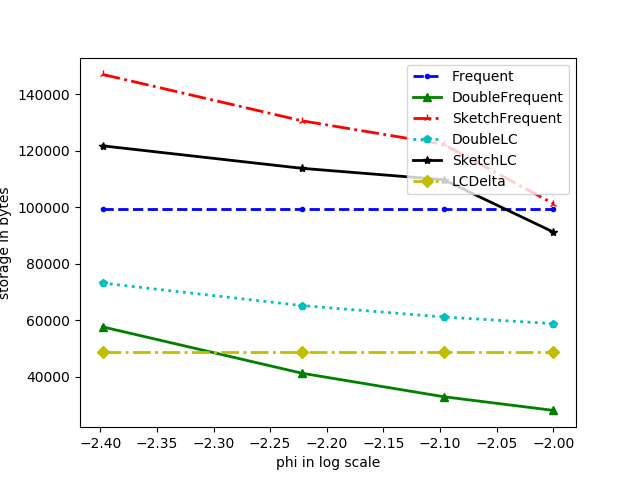
\includegraphics[width=\textwidth]{../Plots/storage_phi.png}
\caption{Planted: Space vs.~$\phi$}
\label{fig:plspphi}
\end{subfigure}
~
\begin{subfigure}[b]{0.33\textwidth}
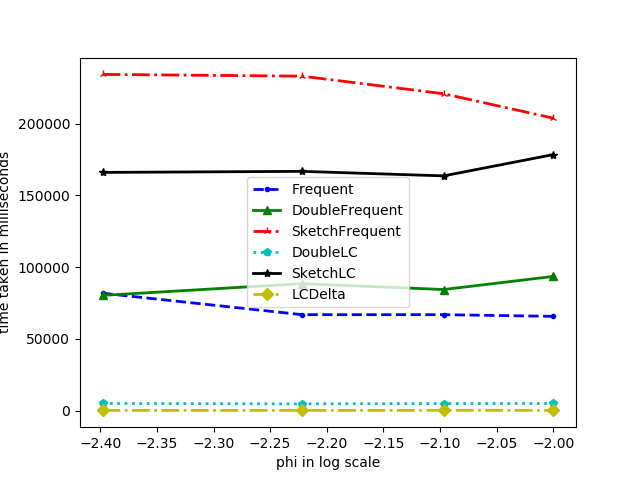
\includegraphics[width=\textwidth]{../Plots/time_phi.png}
\caption{Planted: Update time vs.~$\phi$}
\label{fig:pltimphi}
\end{subfigure}

\begin{subfigure}[b]{0.33\textwidth}
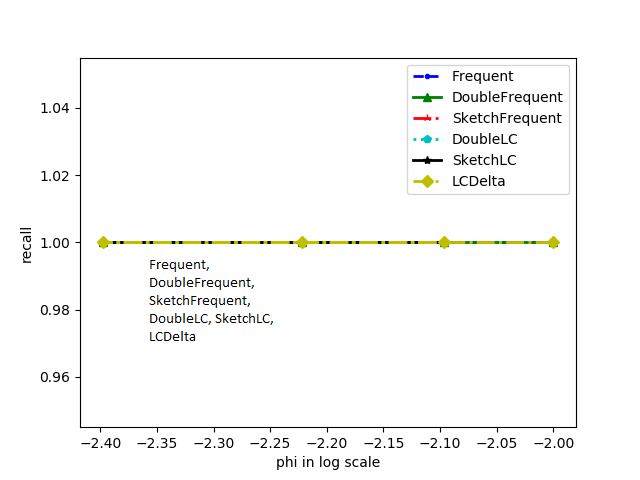
\includegraphics[width=\textwidth]{../Plots/recall_phi.png}
\caption{Planted: Recall vs.~$\phi$}
\label{fig:plrecphi}
\end{subfigure}
~
\begin{subfigure}[b]{0.33\textwidth}
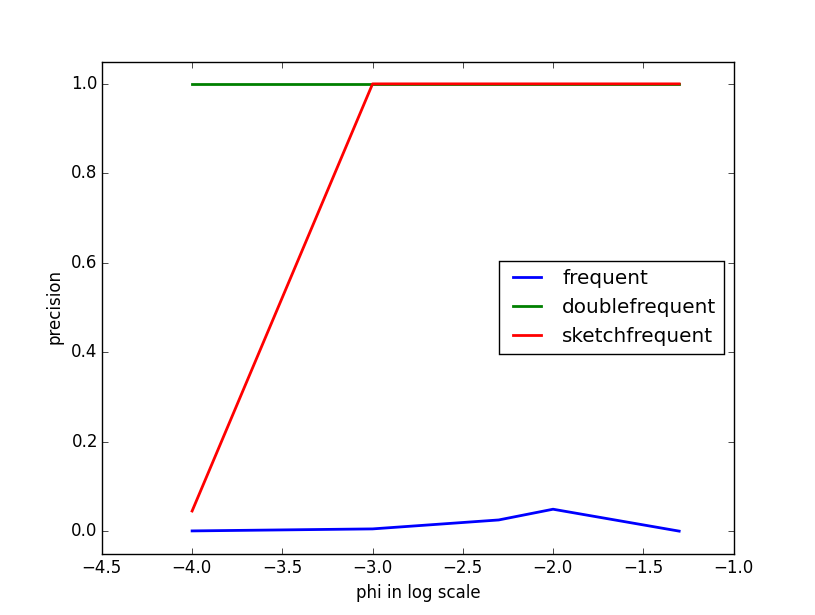
\includegraphics[width=\textwidth]{../Plots/precision_phi.png}
\caption{Planted: Precision vs.~$\phi$}
\label{fig:plprephi}
\end{subfigure}
\caption{Comparison between the algorithms when run on data generated from the planted model. Here, $\eps$ is fixed to $10^{-3}$.}
\label{fig:fixeps}
\end{figure*}

We ran experiments on two sets of synthetically generated data. The first set is generated from a planted distribution where $5$ randomly
chosen elements each constitute $2\%$ of the stream, while the other $n-5$ elements are inserted with uniform probability for the rest $90\%$ of the stream. Here, we
set the universe size $n = 10^5$ and the length of each stream $m=100$. The second set is generated from skewed {Zipfian} distributions, where the skew ranges from $1.2$ to $2$. 
In this case, the streams are drawn from a universe of size $10^5$, while the length of each stream is $16$.  
For both datasets, we varied $\eps$ from $10^{-5}$ to $10^{-2}$ and varied $\phi$ from $0.004$ to $0.01$ (while keeping $\phi \geq \eps$).

Note that although we do not test our algorithms on real-world datasets, the latter can often be approximated with Zipfian distributions. For example, it has been established that sizes of cities and word frequencies in text \cite{zipf}, citations of papers \cite{red98}, web page accesses \cite{bre99}, and file transfer sizes \cite{bes99} have distributions whose tails are bounded by Zipfian distributions. Thus, we can reasonably expect that the results of our experiments on the Zipfian dataset capture some behavior that would be observed in reality.

The algorithms are compared below according to the following attributes:
\begin{itemize}
\item
\textbf{Space}: Storage space used, measured in bytes
\item
\textbf{Update time}: Time take to insert all the items in the stream, measured in milliseconds
\item
\textbf{Recall}: number of true heavy hitters reported, divided by the total number of true heavy hitters.
\item
\textbf{Precision}:number of true heavy hitters reported, divided by the total number of items reported.
\end{itemize}
For each of the above, we performed 5 runs per experiment.

\subsection{Planted Data}




First, we present results for the dataset generated using the planted model. We investigated how the different algorithms fare
against each other as we vary the parameters $\phi$ and $\eps$. Figure \ref{fig:fixeps} shows the data when $\eps=0.001$ and $\phi$
is varied, while Figure \ref{fig:fixphi} is for $\phi=0.01$ and $\eps$ varying.

Consider the case when $\phi$ is varied. Figure \ref{fig:plspphi} shows that as $\phi$ becomes larger, \textsc{DoubleFrequent} uses the least space.
Second in the race is \textsc{LCDelta} which beats out \textsc{DoubleLC}. \textsc{Frequent} and the algorithms using sketches need at least $50\%$ 
more space. In terms of update time, Figure \ref{fig:pltimphi} shows that \textsc{LCDelta} and \textsc{DoubleLC} are far more efficient than the rest,
while those two are comparable. Figures \ref{fig:plrecphi} and \ref{fig:plprephi} show that all the algorithms achieve perfect recall and precision for this setting of parameters.

Now, we turn to Figure \ref{fig:fixphi} where $\eps$ is varied as $\phi$ is kept at 0.01. The range over which $\eps$ is varied is much bigger ($10^{-5}$ to $10^{-2}$) than the range over which $\phi$ was varied in Figure \ref{fig:fixeps}, so here, we see a more high-level view of the algorithms' behavior. As $\eps$ becomes small, the algorithm taking the least amount of space is \textsc{DoubleFrequent} followed by \textsc{LCDelta} and \textsc{DoubleLC} (Figure \ref{fig:plspeps}). Note that when $\eps$ is not much smaller than $\phi=0.01$, all the algorithms have roughly the same space usage.  In terms of update time (Figure \ref{fig:pltimeps}), again as above, \textsc{LCDelta} and \textsc{DoubleLC} have by far the best performance, whether for small or large $\eps$. For precision and recall (Figures \ref{fig:plreceps} and \ref{fig:plpreeps}), all the algorithms have perfect precision and recall\footnote{Except for one datapoint at $\eps=10^{-5}$ in Figure \ref{fig:plreceps} which we believe is due to the probabilistic nature of \textsc{DoubleLC}}.

Overall, we see that \textsc{DoubleFrequent} has the best performance in terms of space, although its updates are slow compared to \textsc{LCDelta} and \textsc{DoubleLC}. Surprisingly, for our planted dataset, \textsc{DoubleLC} does not offer any advantages over \textsc{LCDelta}. The algorithms using sketching, \textsc{SketchFrequent} and \textsc{SketchLC}, are expensive in terms of both time and space. 
\begin{figure*}
\centering
\begin{subfigure}[b]{0.33\textwidth}
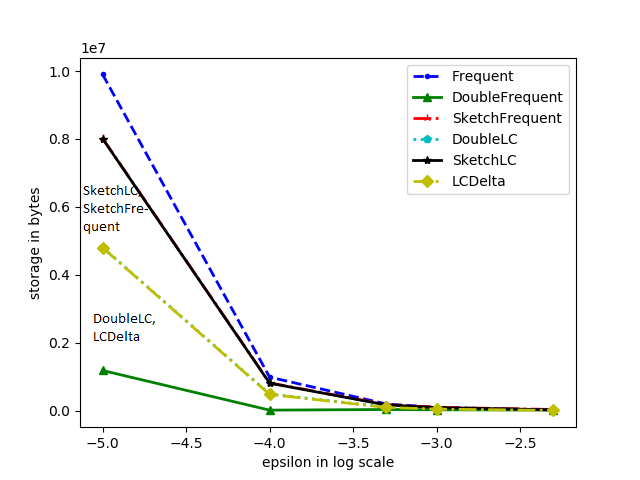
\includegraphics[width=\textwidth]{../Plots/storage_epsilon.png}
\caption{Planted: Space vs.~$\eps$}
\label{fig:plspeps}
\end{subfigure}
~
\begin{subfigure}[b]{0.33\textwidth}
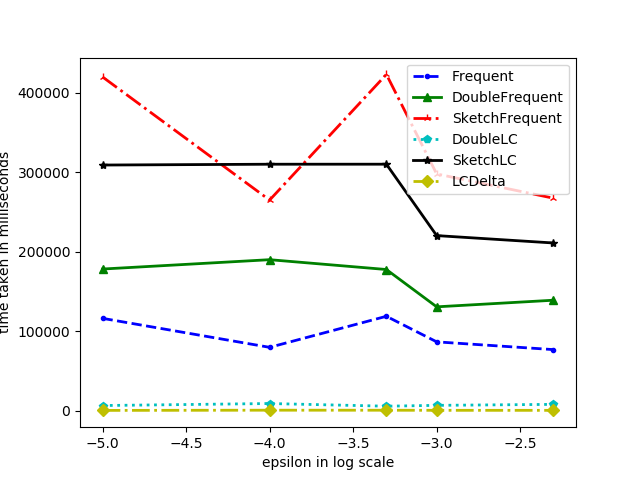
\includegraphics[width=\textwidth]{../Plots/time_epsilon.png}
\caption{Planted: Update time vs.~$\eps$}
\label{fig:pltimeps}
\end{subfigure}

\begin{subfigure}[b]{0.33\textwidth}
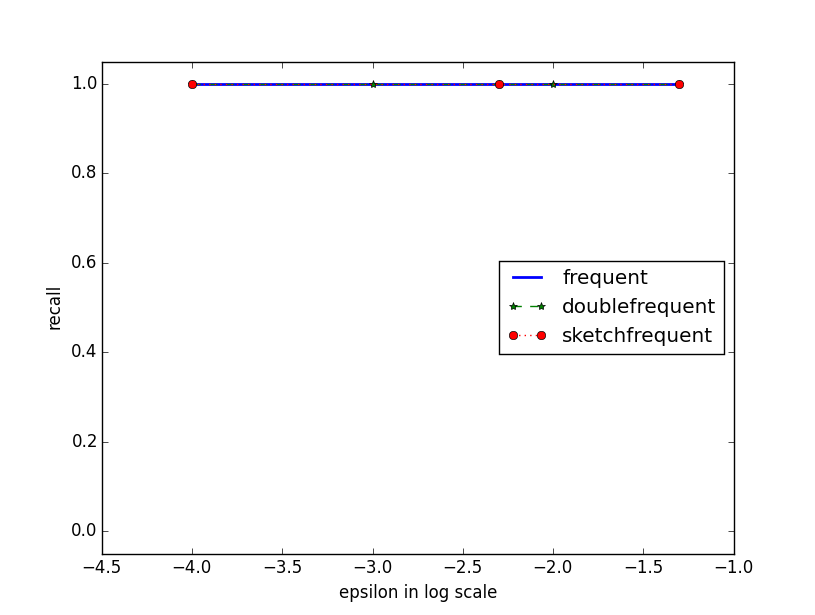
\includegraphics[width=\textwidth]{../Plots/recall_epsilon.png}
\caption{Planted: Recall vs.~$\eps$}
\label{fig:plreceps}
\end{subfigure}
~
\begin{subfigure}[b]{0.33\textwidth}
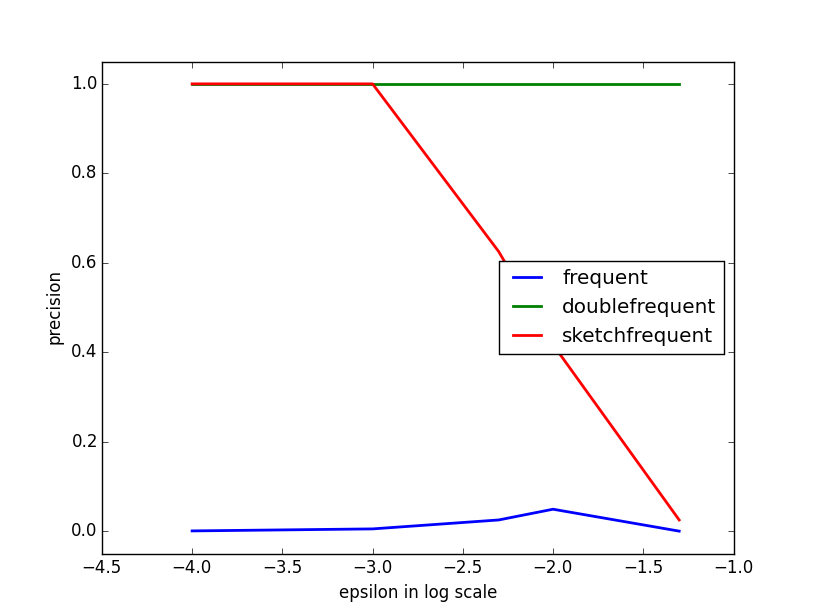
\includegraphics[width=\textwidth]{../Plots/precision_epsilon.png}
\caption{Planted: Precision vs.~$\eps$}
\label{fig:plpreeps}
\end{subfigure}
\caption{Comparison between the algorithms when run on data generated from the planted model. Here, $\phi$ is fixed to $10^{-2}$.}
\label{fig:fixphi}
\end{figure*}

\subsection{Zipfian Data}
\begin{figure*}[b]
\centering
\begin{subfigure}[b]{0.3\textwidth}
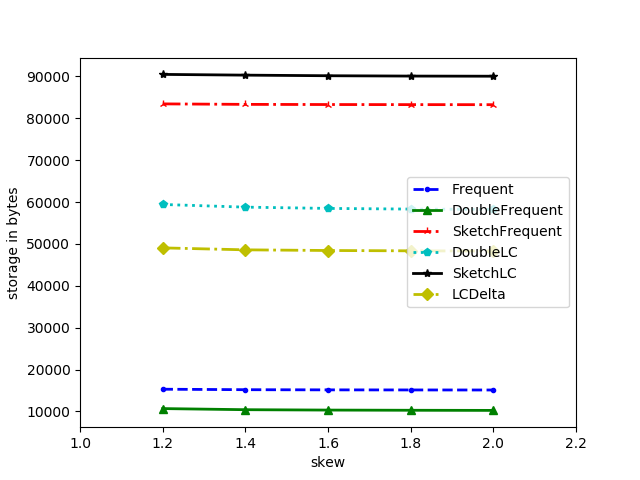
\includegraphics[width=\textwidth]{../Plots/storage_skew.png}
\caption{Zipf: Space vs.~skew}
\end{subfigure}
~
\begin{subfigure}[b]{0.3\textwidth}
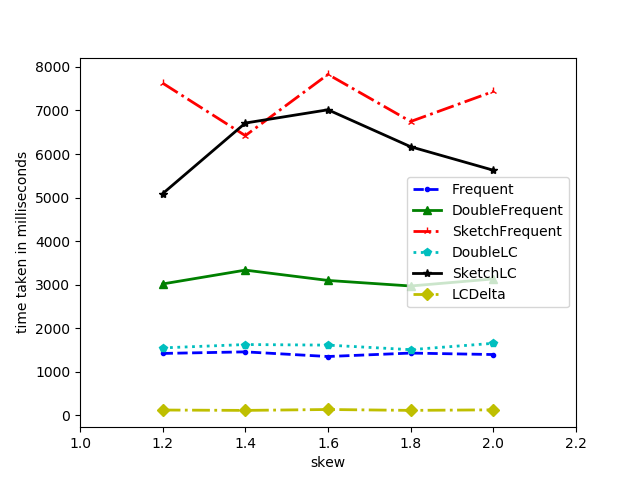
\includegraphics[width=\textwidth]{../Plots/time_skew.png}
\caption{Zipf: Update time vs.~skew}
\end{subfigure}

\begin{subfigure}[b]{0.3\textwidth}
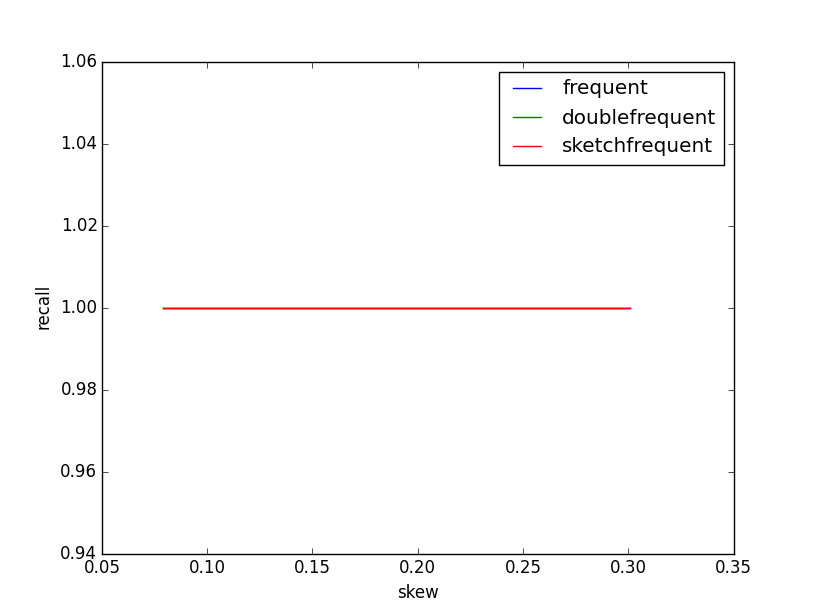
\includegraphics[width=\textwidth]{../Plots/recall_skew.png}
\caption{Zipf: Recall vs.~skew}
\end{subfigure}
~
\begin{subfigure}[b]{0.3\textwidth}
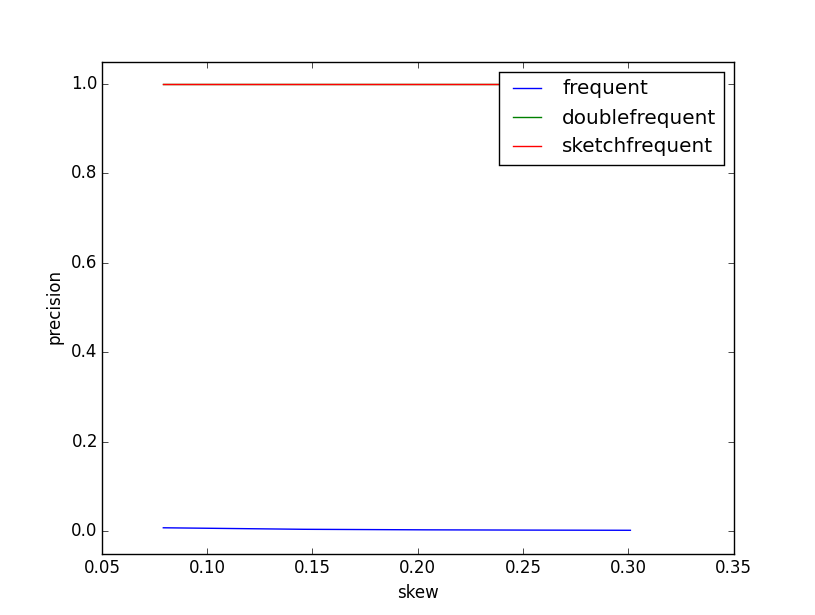
\includegraphics[width=\textwidth]{../Plots/precision_skew.png}
\caption{Zipf: Precision vs.~skew}
\end{subfigure}
\caption{Comparison between the algorithms when run on Zipfian data. Skew varies as $\eps = 0.001$ and $\phi = 0.01$.}
\end{figure*}

Next, we present results for the Zipfian data. 

\begin{figure*}
\centering
\begin{subfigure}[b]{0.3\textwidth}
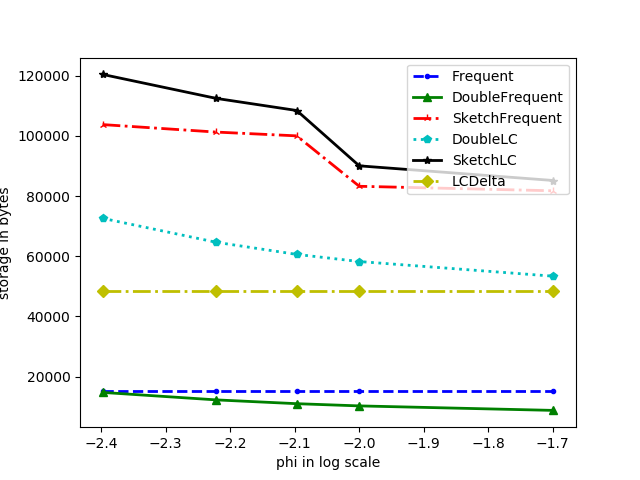
\includegraphics[width=\textwidth]{../Plots/storage_phiskew.png}
\caption{Zipf: Space vs.~$\phi$}
\end{subfigure}
~
\begin{subfigure}[b]{0.3\textwidth}
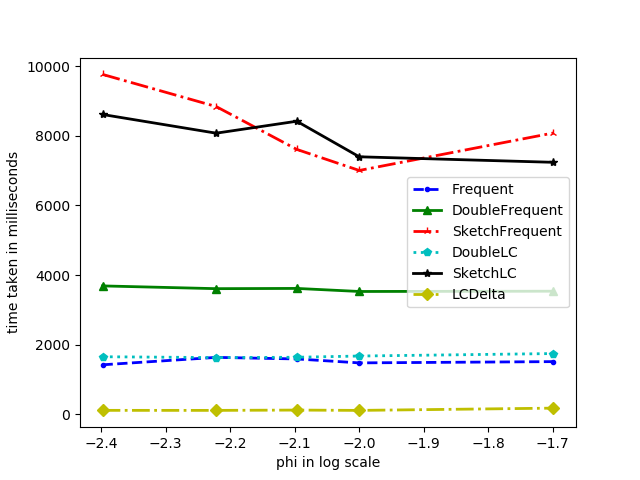
\includegraphics[width=\textwidth]{../Plots/time_phiskew.png}
\caption{Zipf: Update time vs.~$\phi$}
\end{subfigure}

\begin{subfigure}[b]{0.3\textwidth}
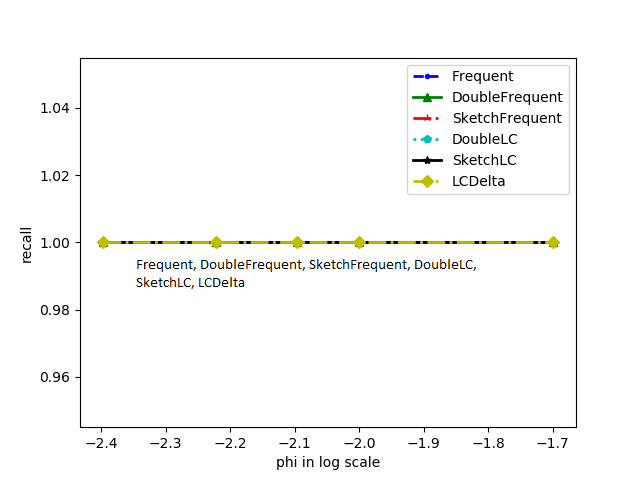
\includegraphics[width=\textwidth]{../Plots/recall_phiskew.png}
\caption{Zipf: Recall vs.~$\phi$}
\end{subfigure}
~
\begin{subfigure}[b]{0.3\textwidth}
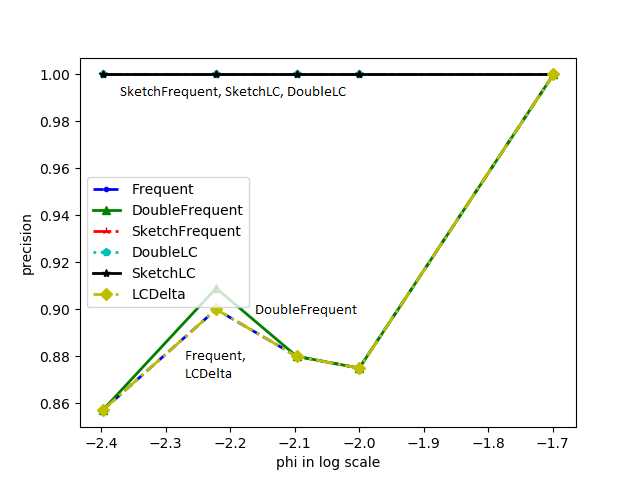
\includegraphics[width=\textwidth]{../Plots/precision_phiskew.png}
\caption{Zipf: Precision vs.~$\phi$}
\end{subfigure}
\caption{Comparison between the algorithms when run on Zipfian data. $\phi$ varies as $\eps = 0.001$ and $\text{skew} = 2$.}
\end{figure*}

\begin{figure*}
\centering
\begin{subfigure}[b]{0.3\textwidth}
\includegraphics[width=\textwidth]{../Plots/storage_epsilonskew.png}
\caption{Zipf: Space vs.~$\phi$}
\end{subfigure}
~
\begin{subfigure}[b]{0.3\textwidth}
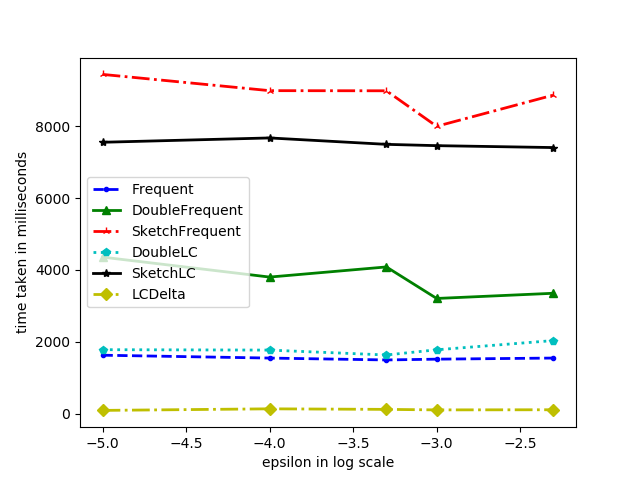
\includegraphics[width=\textwidth]{../Plots/time_epsilonskew.png}
\caption{Zipf: Update time vs.~$\phi$}
\end{subfigure}

\begin{subfigure}[b]{0.3\textwidth}
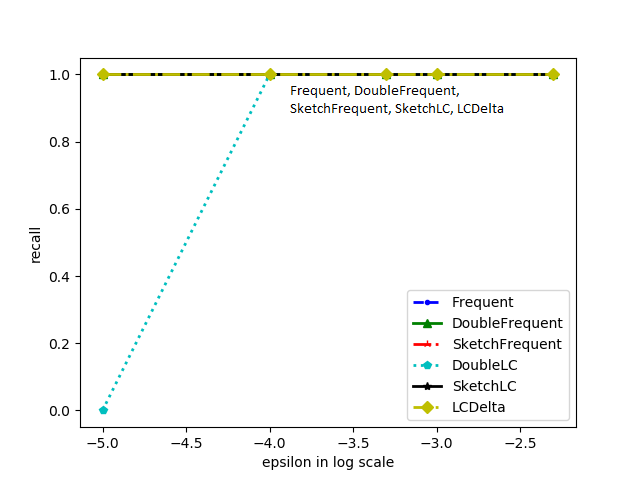
\includegraphics[width=\textwidth]{../Plots/recall_epsilonskew.png}
\caption{Zipf: Recall vs.~$\phi$}
\end{subfigure}
~
\begin{subfigure}[b]{0.3\textwidth}
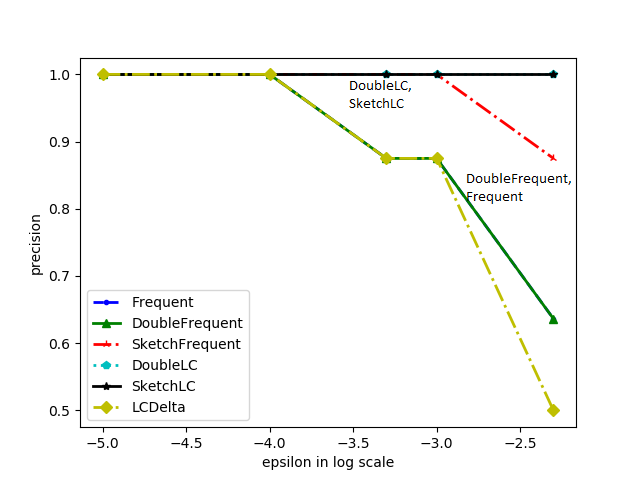
\includegraphics[width=\textwidth]{../Plots/precision_epsilonskew.png}
\caption{Zipf: Precision vs.~$\phi$}
\end{subfigure}
\caption{Comparison between the algorithms when run on Zipfian data. $\epsilon$ varies as $\phi = 0.01$ and $\text{skew} = 2$.}
\end{figure*}



\section{Future Work}

\clearpage
%
% The next two lines define the bibliography style to be used, and the bibliography file.
\bibliographystyle{ACM-Reference-Format}
\bibliography{papers}

% 
% If your work has an appendix, this is the place to put it.
\end{document}
